\begin{frame}
    \centering \Huge Jet validation \\ An introduction
\end{frame}

\begin{frame}{What is validation}
    \begin{itemize}
        \item Necessary to make sure that the switch to r22 is correctly done
        \item Starting point were representative r21 MC samples for each group
        \item Format: Events to Hits to AOD to DAOD\_PHYSVAL to NTUP\_PHYSVAL
        \item NTUP\_PHYSVAL is just a histogram format useful for comparison
        \item Downloaded and overlaid plots are being created, evaluated and investigated
    \end{itemize}
\end{frame}

\begin{frame}{An example}
    \begin{itemize}
        \item Validation of jet reconstruction using FlowElements instead of PFO for release 22
        \item Sample: JZ7 
        \item Collections: AntiKt4EMPFlowJets, AntiKt4EMPFlowFEJets
    \end{itemize}
    \begin{figure}
        \centering
        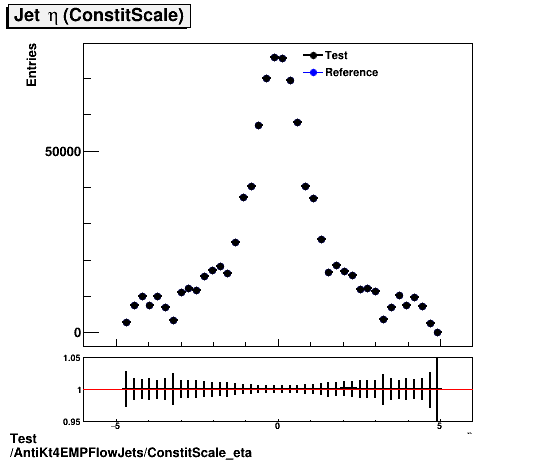
\includegraphics[width=0.64\textwidth]{goodAgreement.png}
    \end{figure}    
\end{frame}

\begin{frame}{Red plots}
    \begin{columns}
        \begin{column}{0.5\textwidth}
            \centering 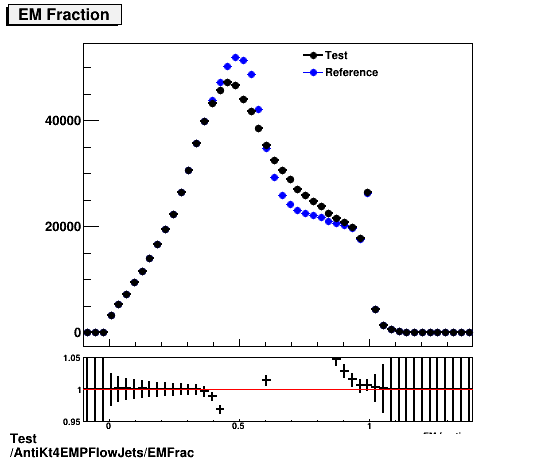
\includegraphics[width=0.72\textwidth]{FEEM}
            \centering 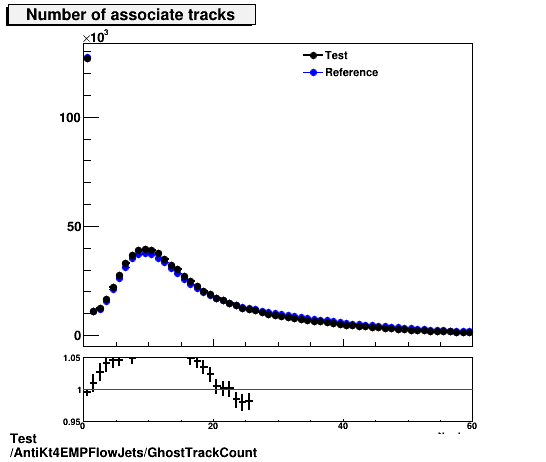
\includegraphics[width=0.72\textwidth]{FEtracks}
        \end{column}
        \begin{column}{0.5\textwidth}
            \centering 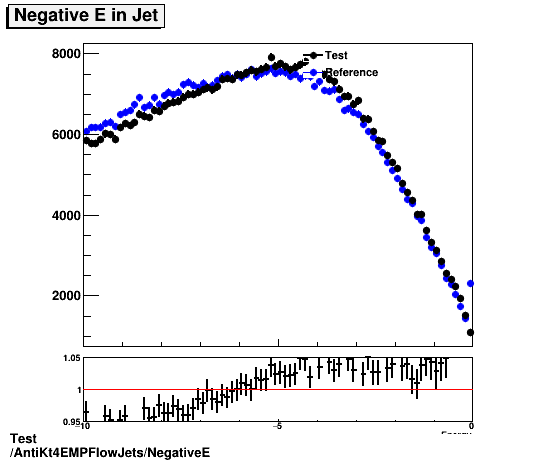
\includegraphics[width=0.72\textwidth]{FEnegE}
            \begin{itemize}
                \item Electromagnetic fraction, negative energy and number of associated tracks show bad agreement.
                \item The reason now has to be investigated
            \end{itemize}
        \end{column}
    \end{columns}
\end{frame}

\begin{frame}{Explanation of the disagreements}
    \begin{block}{Negative energy}
        Explained by the compression of topocluster moments in the AOD. Turning this off leads to perfect agreement.
    \end{block}
    \begin{block}{Number of associated tracks}
        Thinning applied at AOD level leads to TRT hits not being stored. Therefor PFlow had more tracks.
    \end{block}
    \begin{block}{Electromagnetic fraction}
        For very high energy deposits in EMB2 a default value was chosen for PFO.
    \end{block}
\end{frame}

